\section{Appendice}
In quest'ultima sezione viene riportato un esempio di un'immagine in alta definizione presa dal dataset sul quale è stato effettuato il test. L'immagine è la stessa mostrata in figura \textit{13} nella quale è stata eseguita la detection con frammentazione, l'algoritmo di NMS ed è stato infine applicato l'algoritmo di ricostruzione delle labels.\\

I video, presi dalla sfida VisDrone 2019, sui quali è stato effettuato il test per valutare il tracking possono essere visualizzati al seguente link: \url{https://drive.google.com/open?id=1QDJcgdtY6j8H2aSu8DqZ38UxFOC8th_e}. E' da segnalare che in questi video gli oggetti sono stati individuati tramite con le loro labels esatte anziché tramite detections reali.

\begin{figure}[H]
	\centering
	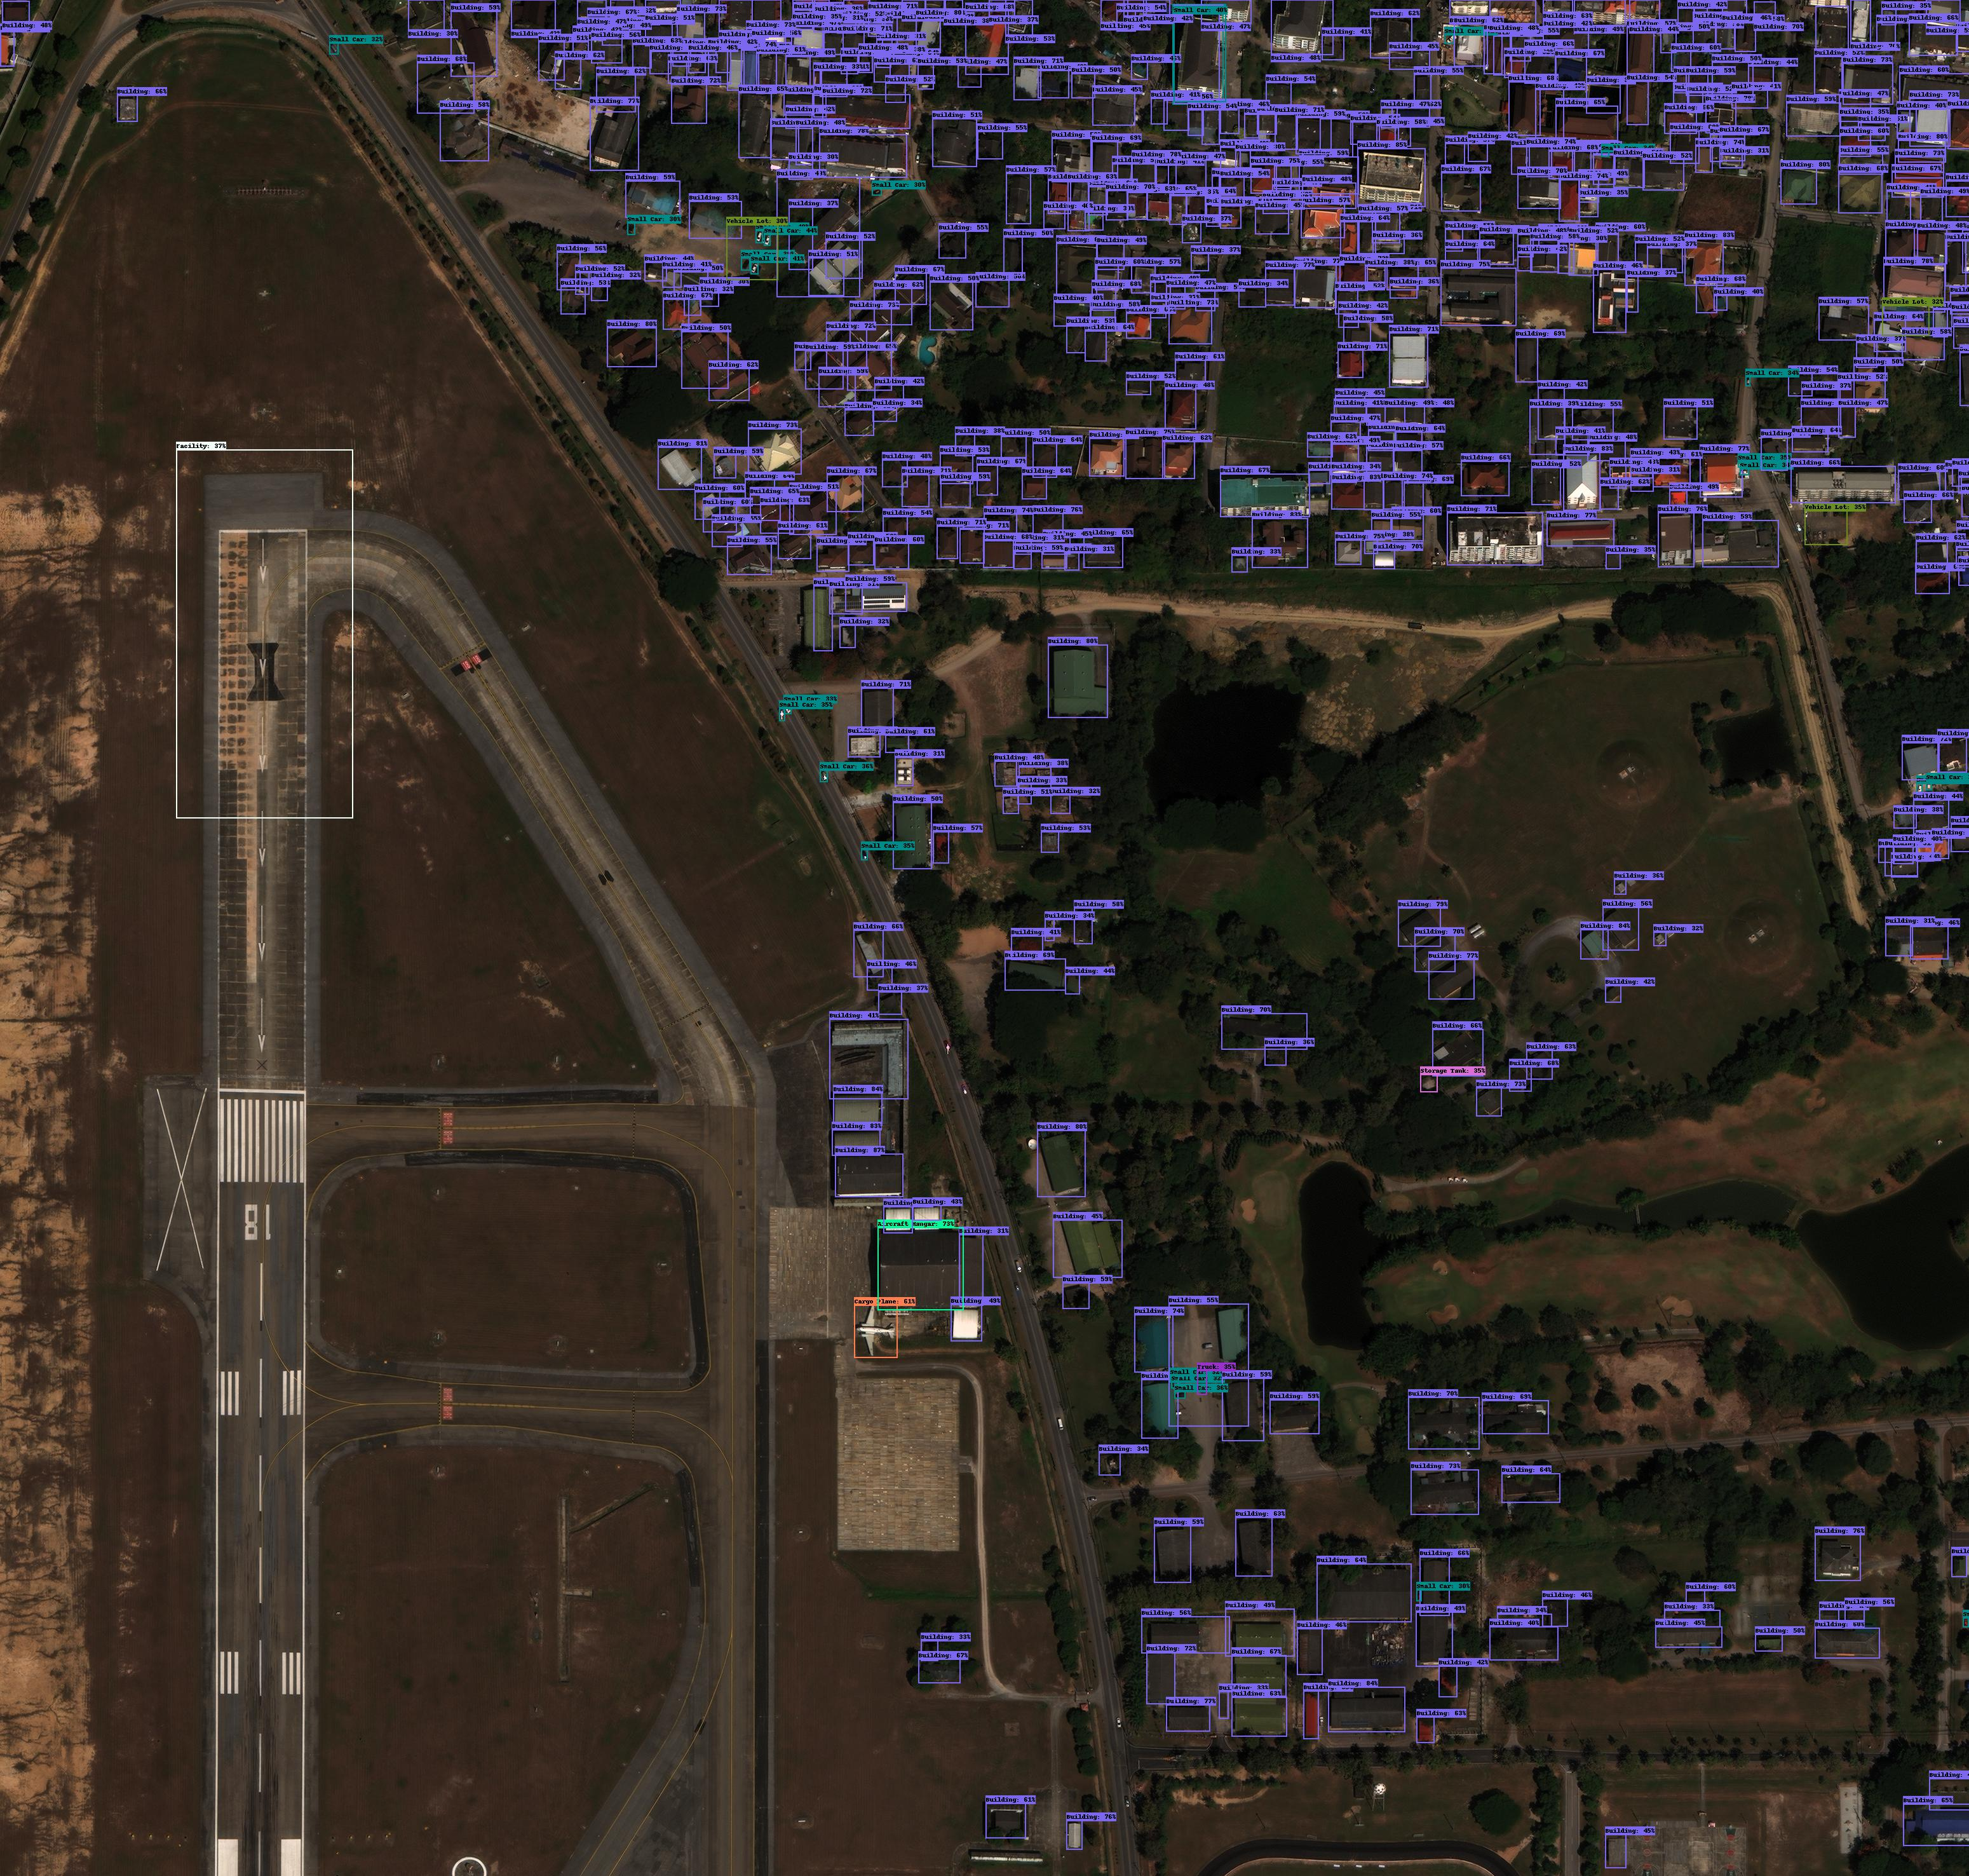
\includegraphics[width=\linewidth]{images/immagine-satellite-detection.jpg}
	\caption{Elaborazione Studiomapp su xView Dataset}
	\label{esempio di immagine con detection e frammentazione}
\end{figure}